\section{Machine Learning}

\begin{itemize}
\item What is machine learning?
\item Supervised learning, i.e.\ have labelled data.
\item Binary classification tasks: Every training example has a label indicating
  the class membership.
\item In HEP, the positive class is typically referred to as \emph{signal} while
  the negative class is referred to as \emph{background}.
\item What is training data, etc.
\item What is training.
\end{itemize}


\subsection{Boosted Decision Trees}

Boosted decision trees (BDT) are a classification algorithm consisting on an
ensemble of \emph{decision tree classifiers} that are combined to yield a more
powerful classifier. The ensemble of decision trees is created using a algorithm
referred to as \emph{boosting}, which iteratively constructs decision tree
classifiers while emphasising training examples that were incorrectly classified
in prior iterations. The following description of BDT focuses on the algorithm
implemented in \textsc{TMVA}~\cite{TMVA}, which is used in this thesis to train
BDT.

The base classifiers used in the boosting algorithm are decision tree
classifiers, which are briefly introduced hereafter. A decision tree partitions
a multivariate space with coordinates $(x_1, \dots, x_n)$ by recursively
performing binary splits along the coordinate axes.






The Gini index is taken an a measure of node impurity, which is defined as
\begin{align*}
  I_{\text{G}} = 2 p (1 - p)
\end{align*}
for a binary classification problem, where $p$ is the purity of training
examples from the signal class in a given node.



The decision tree is constructed in a \emph{greedy} fashion by making







A decision tree is a classification algorithm that partitions

into disjoint

\begin{figure}[htbp]
  \centering

  \begin{subfigure}{0.46\textwidth}
    \centering
    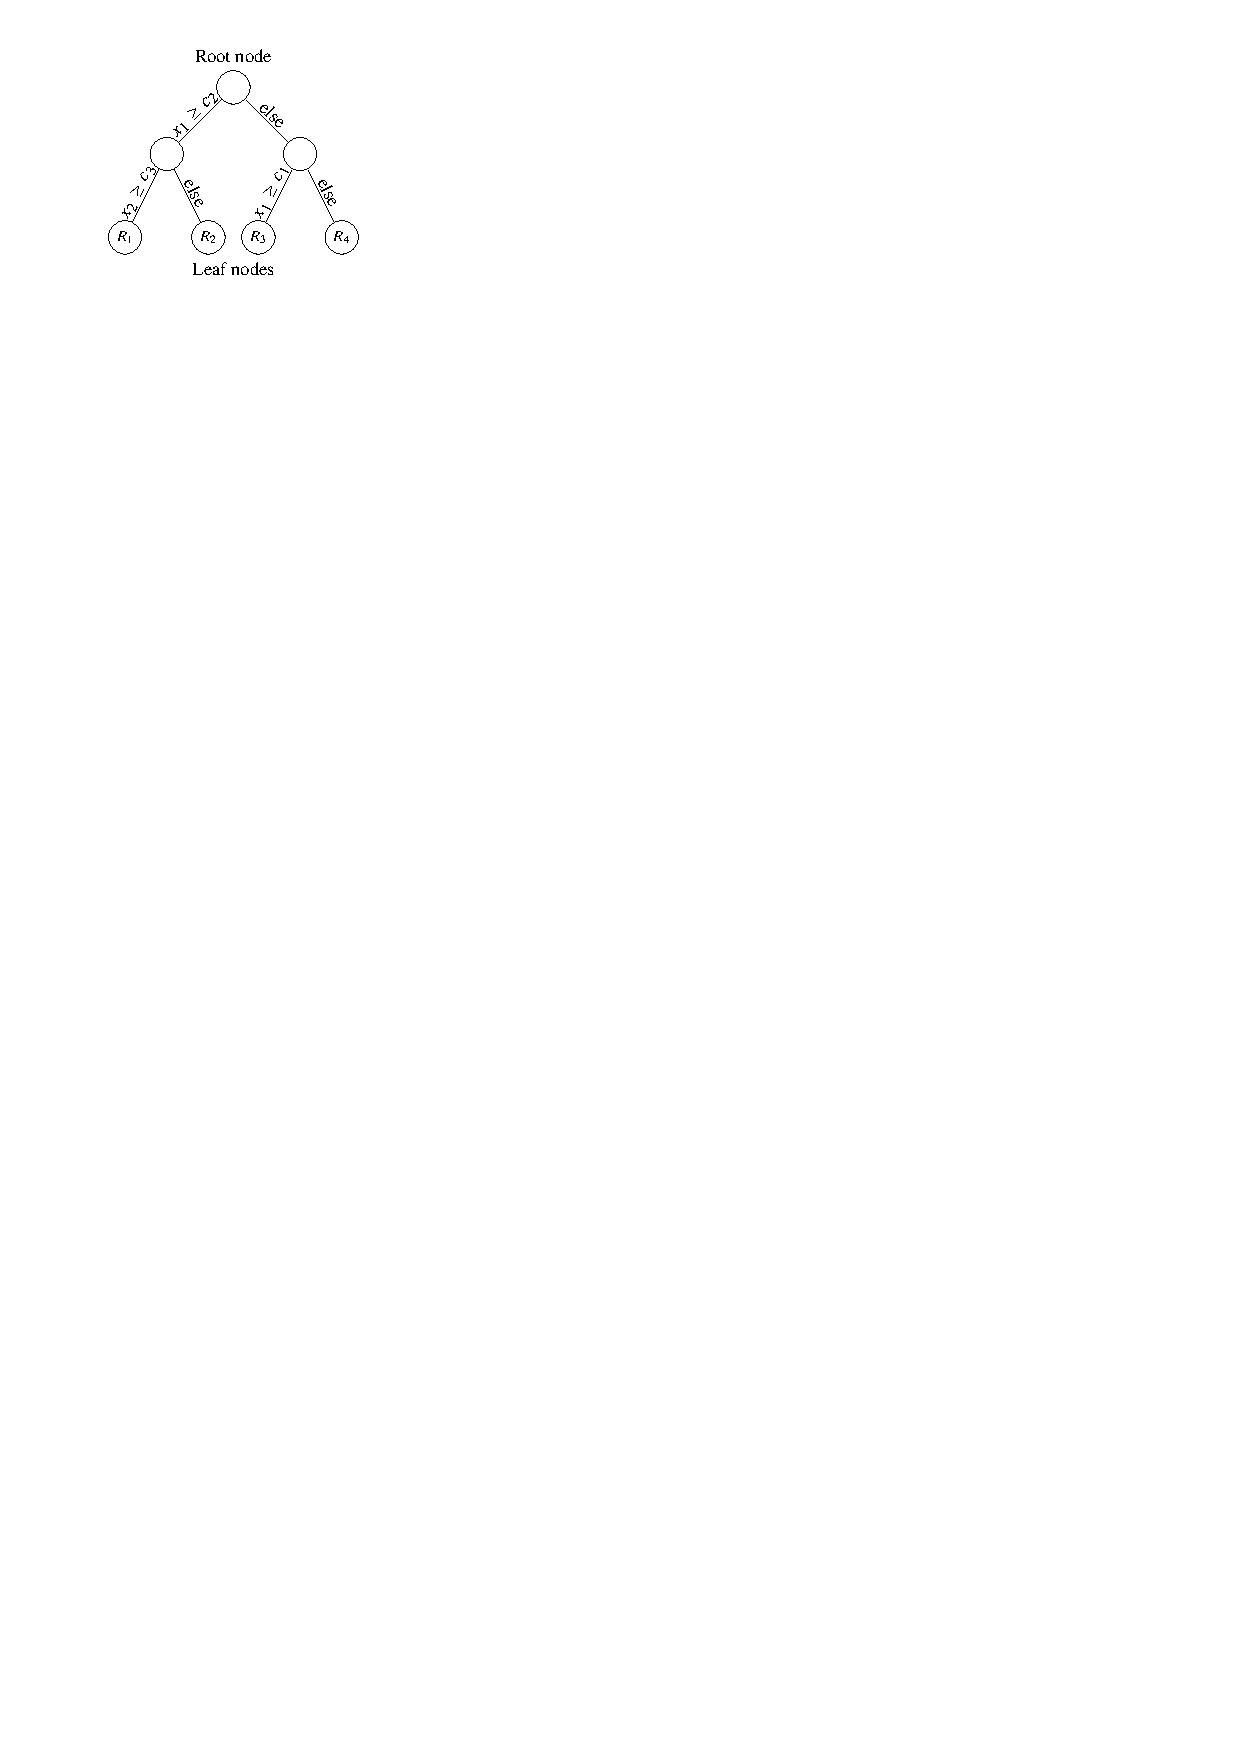
\includegraphics[scale=1.05]{ml/decision_tree}
    \caption{}
  \end{subfigure}\hfill%
  \begin{subfigure}{0.46\textwidth}
    \centering
    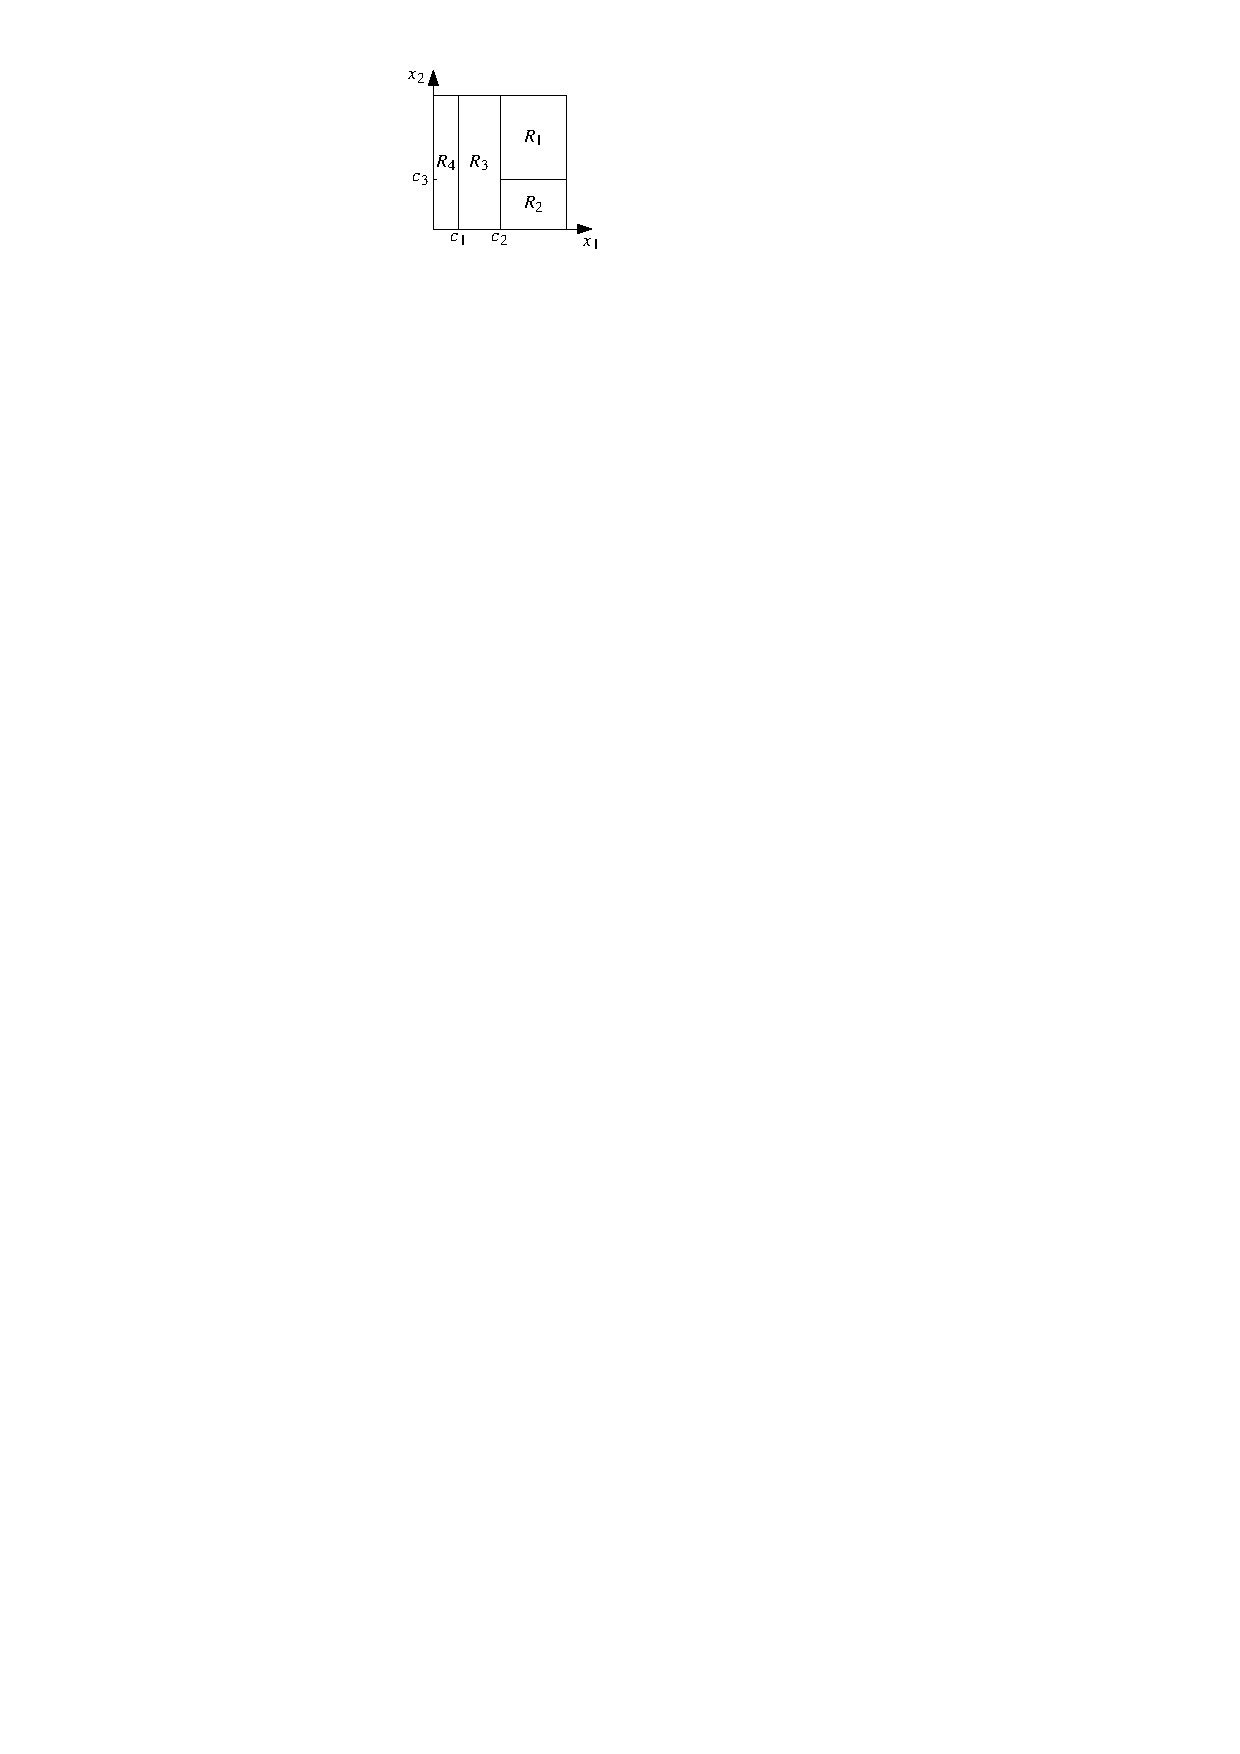
\includegraphics[scale=1.05]{ml/decision_tree_partitioning}
    \caption{}
  \end{subfigure}\hfill%

  \caption{abc. The figure is adapted from Ref.~\cite{hastie09}.}
  \label{fig:decision_tree}
\end{figure}





\subsection{Neural Networks}

\subsubsection{Recurrent Neural Networks}%
\label{sec:rnn}


%%% Local Variables:
%%% mode: latex
%%% TeX-master: "../../phd_thesis"
%%% End:
